\documentclass{beamer}

\title{Machine Learning Analysis on the JET Pedestal Database}

\subtitle{or how I learned to worry about high  $n_e^{ped}$}

\date{9 June, 2021}

\AtBeginSection[]
{
  \begin{frame}
    \frametitle{Table of Contents}
    \tableofcontents[currentsection]
  \end{frame}
}

\usepackage{ulem}
\usepackage{xcolor}

\begin{document}

\frame{\titlepage}


\begin{frame}
	\frametitle{Overview}
	\tableofcontents
\end{frame}

\section{JET Pedestal Database}
\begin{frame}{fragile}
\frametitle{JET pedestal database contains 3000+ entries of H-mode, pre-ELM plasmas}
\begin{columns}

\column{0.33\textwidth}
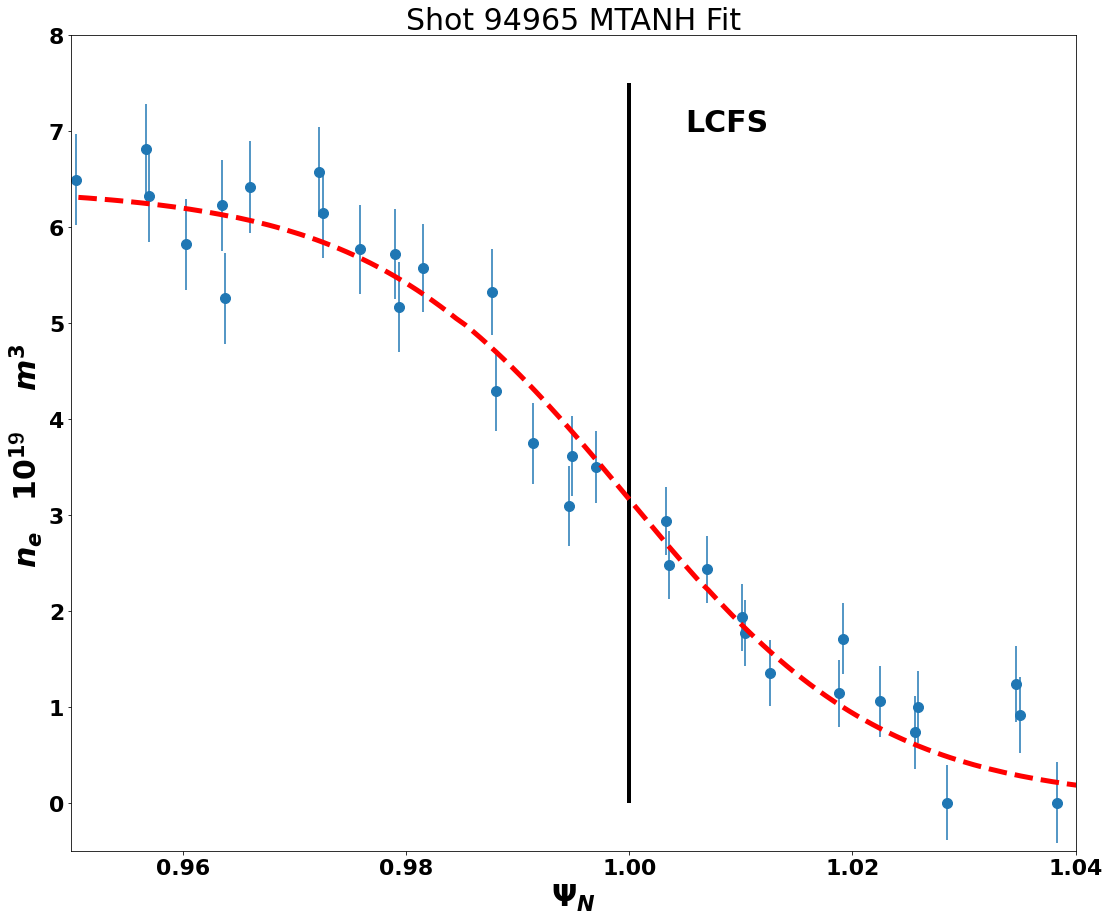
\includegraphics[scale=0.2]{./src/MTANH_fit_21}\hfill
\column{0.2\textwidth}
\column{0.33\textwidth}
\begin{itemize}
	\item Pedestal parameters determined from mtanh fit
	\item Focus on $n_e^{ped}$ height
\end{itemize}
\end{columns}

\end{frame}
\begin{frame}
\frametitle{Use only main engineering parameters to predict $n_e^{ped}$}
\begin{columns}

\column{0.2\textwidth}

\begin{center}
\begin{tabular}{| c | c | }
	\hline
	Eng. Param & Domain \\
	\hline
	$I_P$ [MA] & $[0.81, 4.48]$ \\
	$B_T$ [MW] & $[0.97, 3.68]$ \\
	$a$ [m] & $[0.83, 0.97]$ \\
	$R$ [m] & $[2.8, 2.975]$ \\ 
	$\delta$ [-] & $[0.16, 0.48]$ \\
	$M_{eff}$ [-] & $[1.0, 2.18]$ \\
	$P_{NBI}$ [MW] & $[10^{-3}, 32.34]$ \\
	$P_{ICRH}$ [MW] & $[0, 7.96]$ \\
	$P_{TOT}$ [MW] & $[3.4, 38.22]$ \\
	$V_P$ [m$^3$] &  $[58.3, 82.19]$ \\
	$q_{95}$ [-] & $[2.42, 6.04]$ \\
	$\Gamma$ [$10^{22}$ e/s] & $[0, 15.5]$ \\
	$H$ [-] & $[0, 0.18]$ \\
	$P_{SD}$ [$10^{22}$ e/s] & $[0, 1000]$ \\
	$DC$ [-] & $[VV \cdots]$ \\
	\hline
\end{tabular}
	\end{center}
	\column{0.2\textwidth}\hfill
\column{0.6\textwidth}
\begin{center}
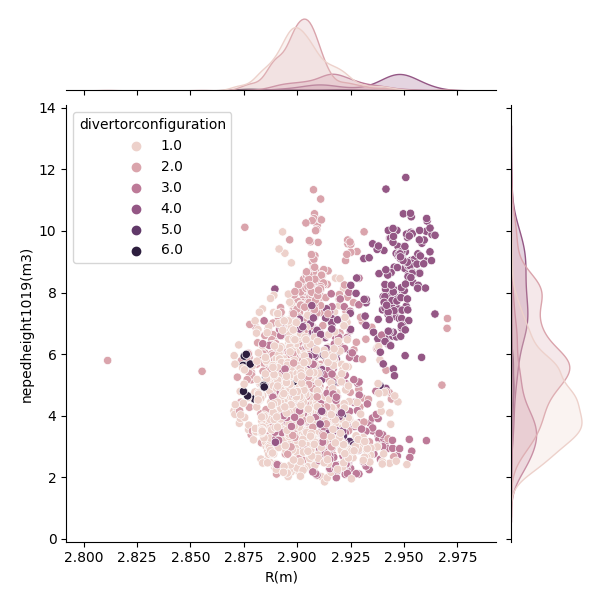
\includegraphics[scale=0.48]{./src/R_vs_NEPED_DC}<1>
\end{center}

\end{columns}
\end{frame}

\begin{frame}
\frametitle{Take only deuterium shots, no RMPs, kicks, or pellets, and remove $R, P_{SD}, DC$ from input space}
\begin{columns}
\column{0.5\textwidth}
\begin{itemize}
	\item Shafranov Shift$\rightarrow$ remove $R$
	\item $P_{SD}$ varies too much. 
	\item Only numerical columns used as input
	\item HRTS Validated 
\end{itemize}

\column{0.50\textwidth}
\begin{tabular}{| c | c | }
	\hline
	Eng. Param & Domain \\
	\hline
	$I_P$ [MA] & $[0.81, 4.48]$ \\
	$B_T$ [MW] & $[0.97, 3.68]$ \\
	$a$ [m] & $[0.83, 0.97]$ \\
	\sout{$\color{red}R \; \text{[m]}$ } & \sout{$ \color{red}[2.8, 2.975]$} \\ 
	$\delta$ [-] & $[0.16, 0.48]$ \\
	$M_{eff}$ [-] & $[1.0, 2.18]$ \\
	$P_{NBI}$ [MW] & $[10^{-3}, 32.34]$ \\
	$P_{ICRH}$ [MW] & $[0, 7.96]$ \\
	$P_{TOT}$ [MW] & $[3.4, 38.22]$ \\
	$V_P$ [m$^3$] &  $[58.3, 82.19]$ \\
	$q_{95}$ [-] & $[2.42, 6.04]$ \\
	$\Gamma$ [$10^{22}$ e/s] & $[0, 15.5]$ \\
	$H$ [-] & $[0, 0.18]$ \\
	\sout{$\color{red} P_{SD} \; [10^{22} \text{e/s}]$} & \sout{$\color{red} [0, 1000]$} \\
	\sout{$\color{red}DC \; [-]$ } & \sout{$\color{red}[VV \cdots]$} \\
	\hline
\end{tabular}

\end{columns}
\end{frame}
\section{Machine Learning}
\begin{frame}
\frametitle{Utilizing more input parameters yeilds higher prediction quality than existing scaling law}
\begin{block}{}
\begin{columns}

\column{0.45\textwidth}
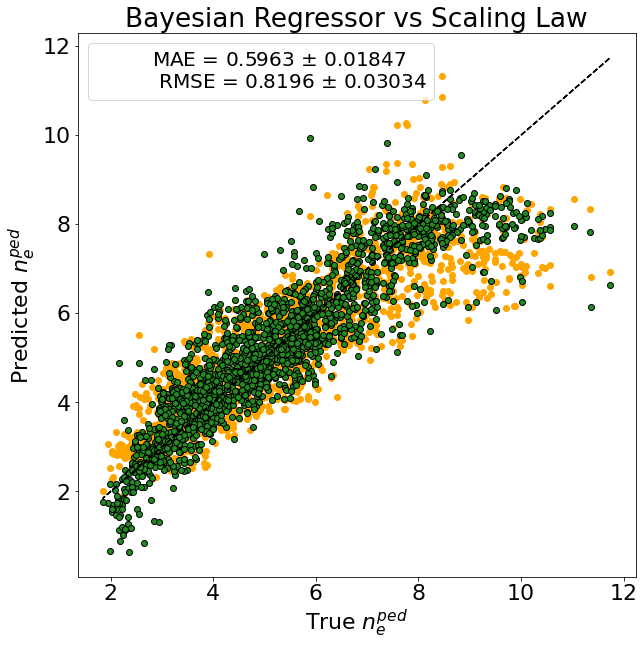
\includegraphics[scale=0.25]{./src/Baysian_regression_predictions}

\column{0.02\textwidth}
\column{0.53\textwidth}
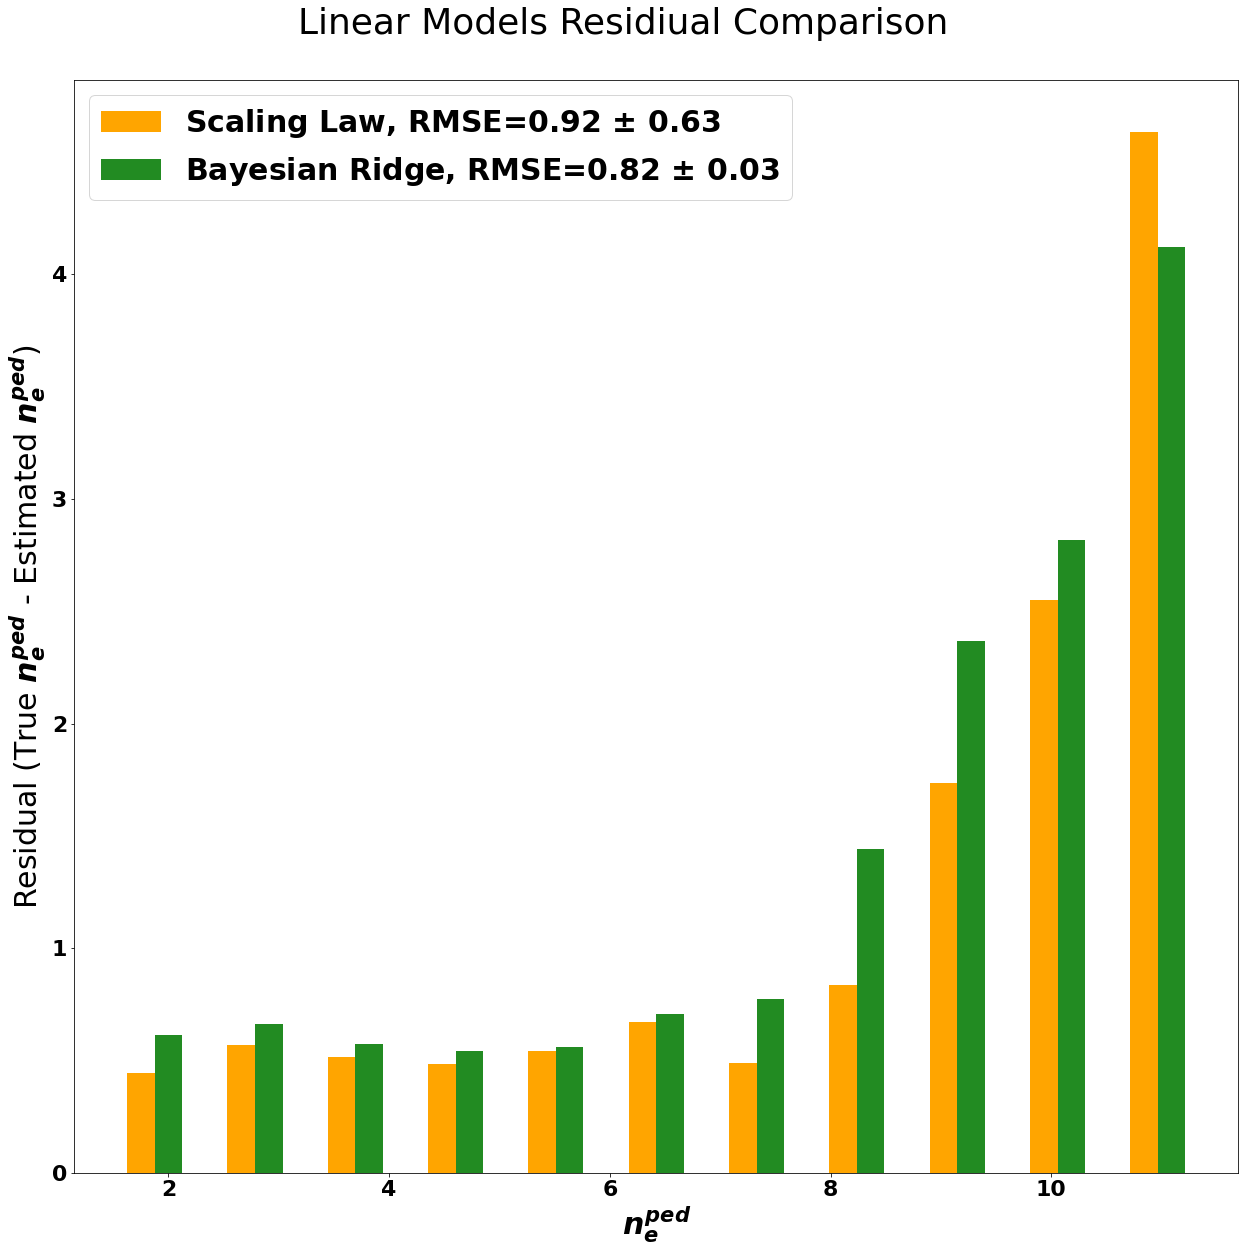
\includegraphics[scale=0.14]{./src/linear_comp}
\end{columns}
\end{block}
\begin{equation}
	n_e^{ped} = (9.9 \pm 0.3) I_p^{1.24 \pm 0.19} P_{TOT}^{-0.34 \pm 0.11} \delta^{0.62 \pm 0.14} \Gamma^{ 0.08 \pm 0.04} M_{eff}^{0.2 \pm 0.2}
\end{equation}

\end{frame}

\begin{frame}
\frametitle{Including more input params reduces interpretability}
\begin{columns}
\column{0.5\textwidth}
\begin{itemize}
	\item Prediction uncertainty \\ normally distributed between 1.6 - 1.8
\end{itemize}
\column{0.5\textwidth}
\begin{tabular}{ | c | c | c |}
			\hline
			Feature & $\mu$ & $\sigma^2$ \\
			\hline
			$I_p$ & 0.15 & 0.06 \\
			$B_T$ & 0.956 & 0.072 \\
			$a$ & 2.966 & 0.479 \\
			$\delta$ & 12.95 & 0.154 \\
			$V_P$ & -0.05 & 0.007 \\
			$q_{95}$ & -1.064 & 0.0542 \\
			$P_{NBI}$ & $-1.911$ & 0.0546 \\
			$P_{ICRH}$ & -1.976 & 0.0561 \\
			$P_{TOT}$ & 1.926 & 0.0557 \\
			$\Gamma$ & 0.125 & 0.007 \\
			$H$ & -4.016 & 0.374  \\
			$M_{eff}$ & 1.369 & 0.053 \\
			\hline
\end{tabular}
\end{columns}
\end{frame}

\begin{frame}
\frametitle{Non-linear models like Random Forests and Extreme Randomized Trees outperform linear models }
\begin{center}
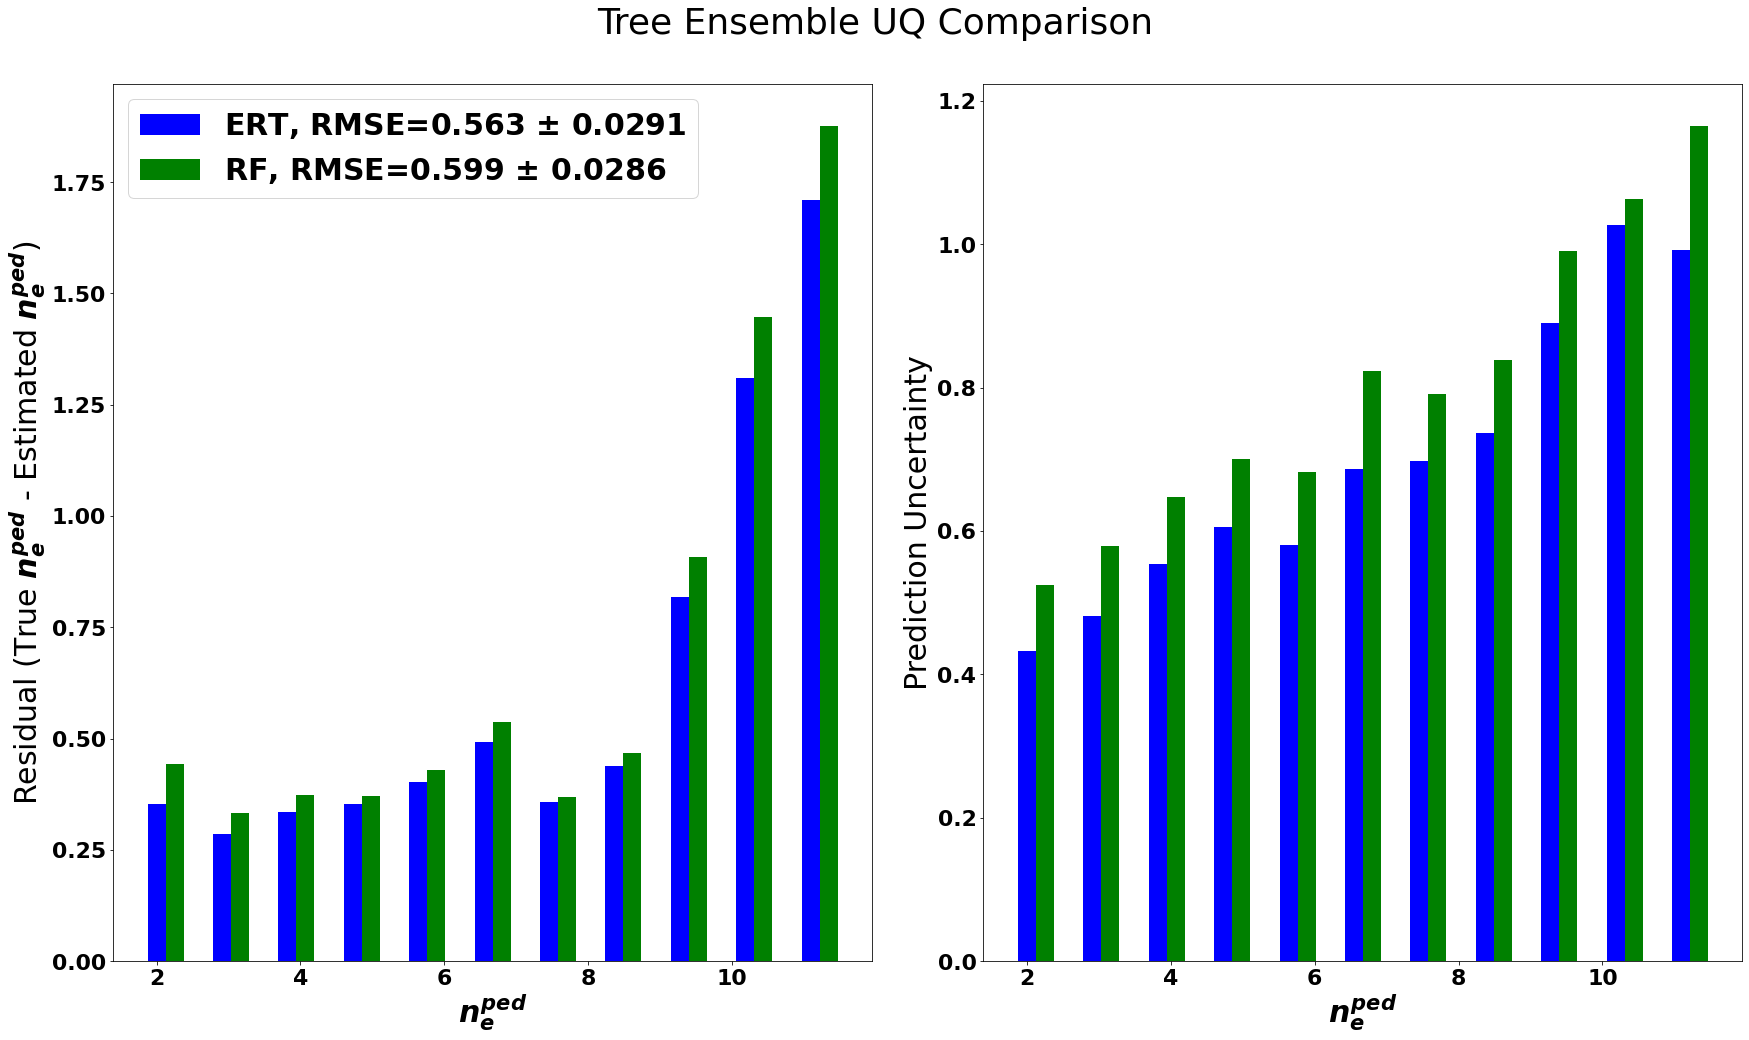
\includegraphics[scale=0.15]{./src/Tree_UQ}
\end{center}

Uncertainty determined from std of each decision tree pred.
\end{frame}

\begin{frame}
\frametitle{Meta-modeling has no effect on RFs and ERTs}
\begin{center}
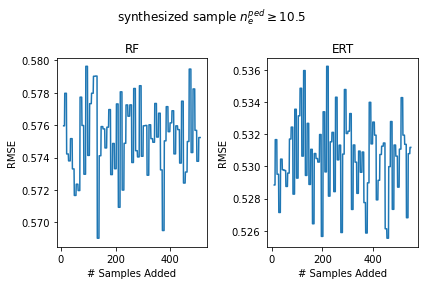
\includegraphics[scale=0.6]{./src/ERT_vs_RF_meta_modeling}
\end{center}
Goes on to 2000+ entries
\end{frame}
\begin{frame}
\frametitle{Can reduce dimensionality for Gaussian Processes using sensitivity analysis $\rightarrow$ remove $H, M_{eff}$ from input space}
\begin{columns}
\column{0.5\linewidth}
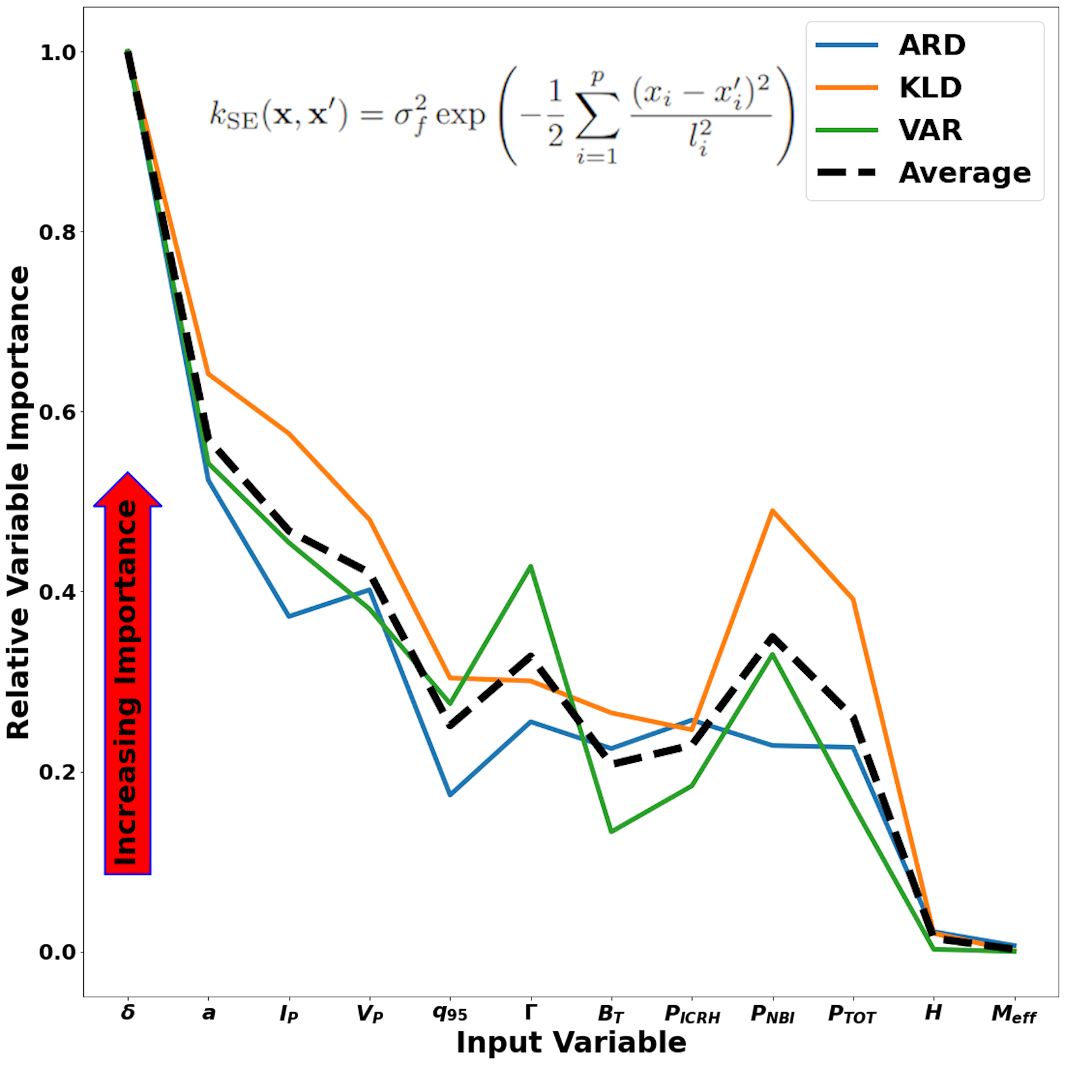
\includegraphics[scale=0.15]{./src/GP_sensitivity_analysis_final_V1_weq}
\column{0.5\linewidth}
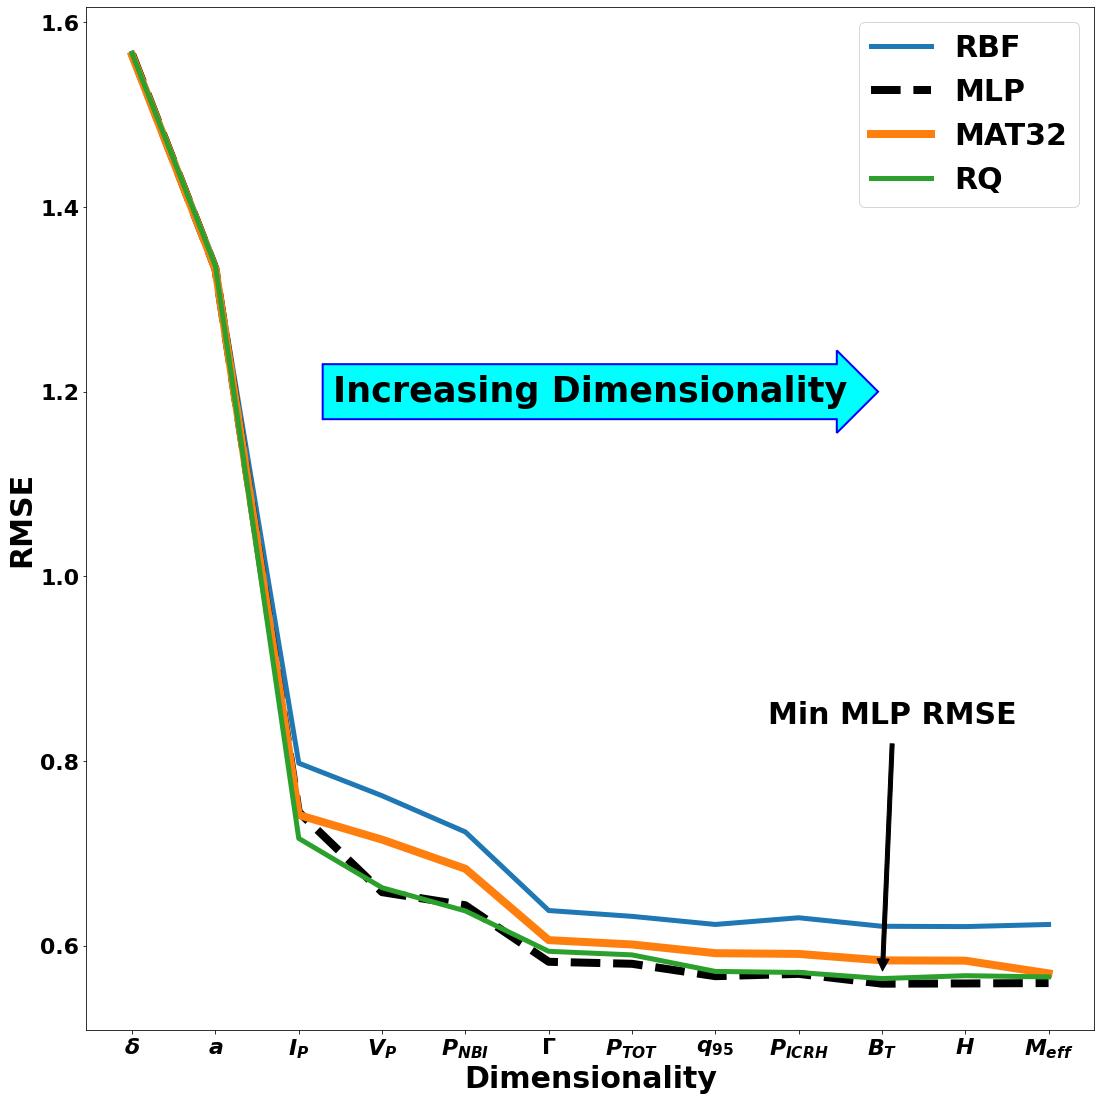
\includegraphics[scale=0.15]{./src/final_GP_dim_v2}
\end{columns}
\end{frame}
\begin{frame}
\frametitle{GPs outpreform RFs and ERTs, and heteroscedastic models can capture local uncertainty}
\begin{figure}
\centering
\includegraphics[scale=0.19]{./src/MLP_UQ_compare}
\end{figure}
\end{frame}

\begin{frame}
\frametitle{Shallow Artifical Neural Networks outperform larger nets}
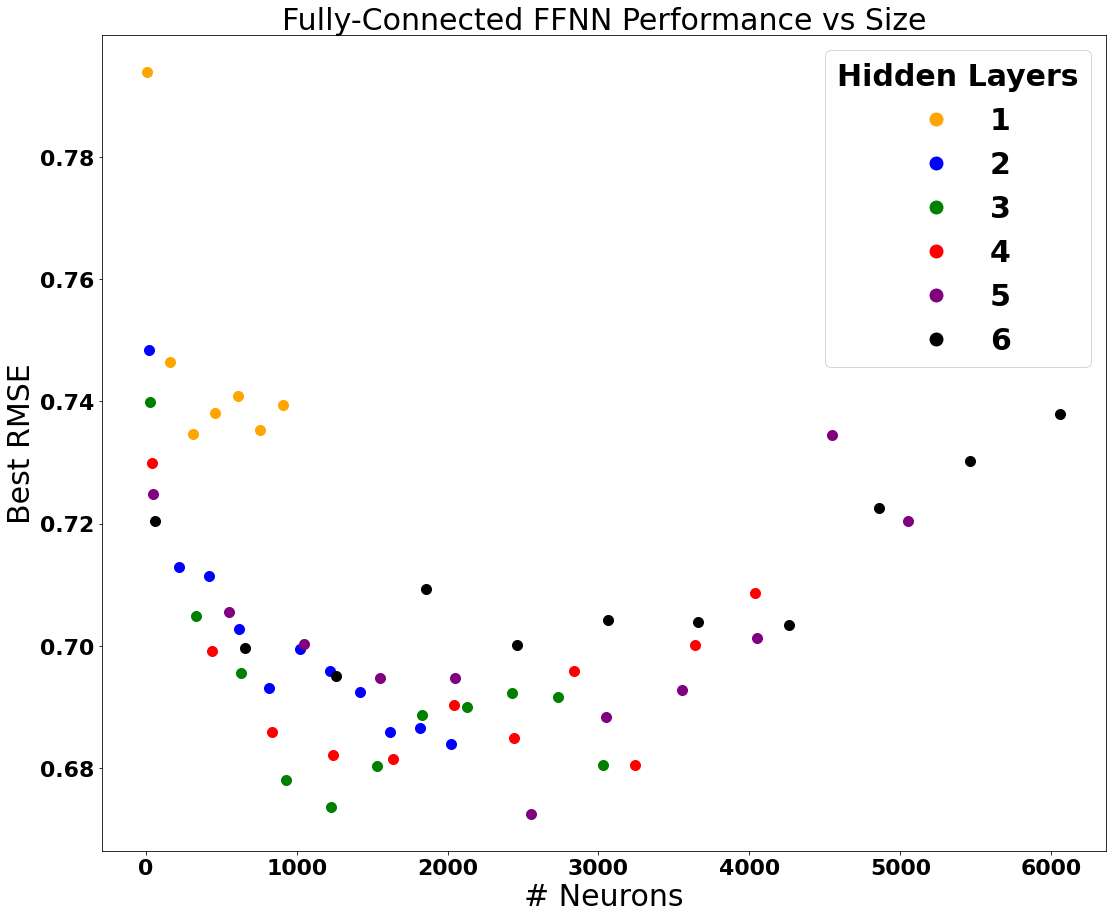
\includegraphics[scale=0.27]{./src/ANN_performace_size}
\end{frame}

\begin{frame}
\frametitle{Ensembling for prediction uncertainty $\rightarrow$ increases with size of ensemble}
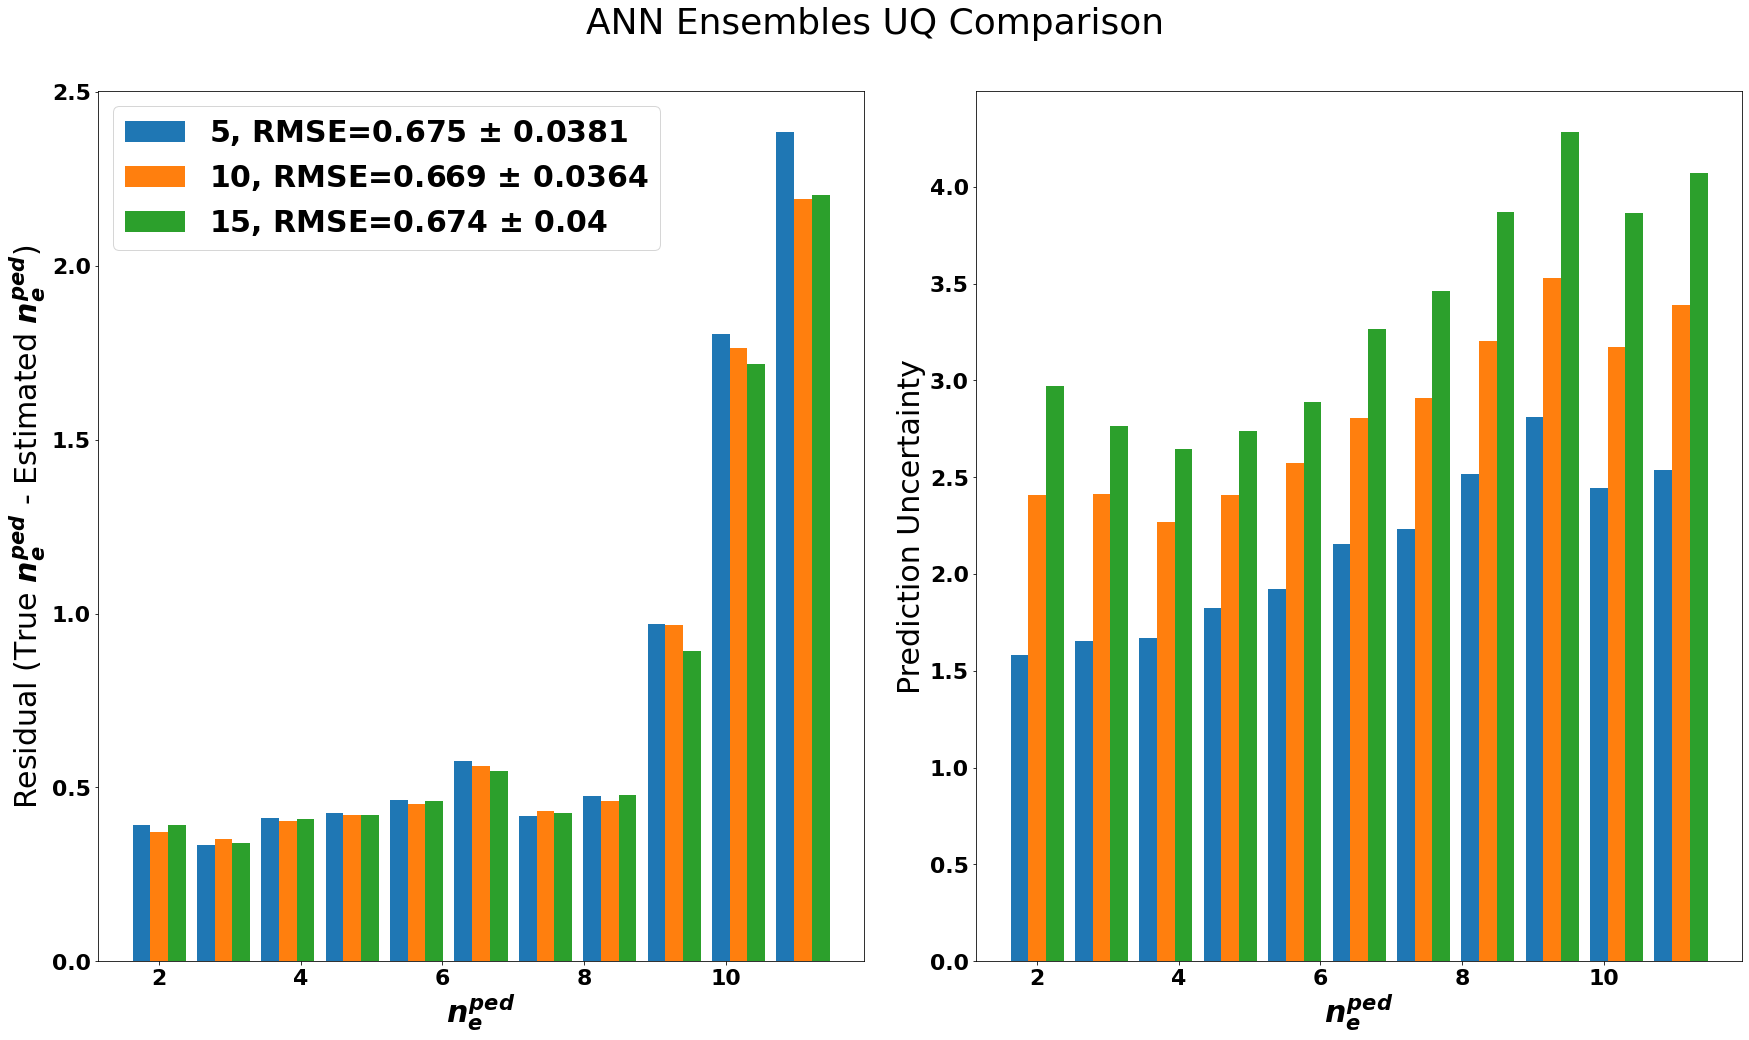
\includegraphics[scale=0.18]{./src/ANN_ensemble_comp}
\end{frame}

\section{Conclusion}
\begin{frame}
\begin{block}{Conclusion}
	\begin{itemize}
		\item Non-linear models outpreform linear models 
		\item RFs and ERTs work well as black box models
		\item Heteroscedastic GPs can map local uncertainty
		\item $n_e^{ped} \geq 9$ is elusive to non-linear models
	\end{itemize}
	\end{block}
	\begin{block}{Future Work}
		\begin{itemize}
			\item Fit models on varied subsets of database
			\item UQ of main engineering parameters
			\item Ideas? 
		\end{itemize}
	\end{block}
\end{frame}

\end{document}
